\chapter{Conclusion}\label{ch:conclusion}
\def \path {intro/}
\def \imgpath {intro/images}

In this thesis, we have examined the effectiveness of using complex wavelets as
basis functions for deep learning models. We summarize the key results we have
found before describing what we were not able to explore due to time constraints.

% We first looked at ScatterNets, a type
% of feature extractor that builds invariances using the complex magnitude
% operation, demodulating image energy towards zero. Having examined the
% properties of these ScThen we looked at a method
% that does not rely on demodulation, and simply learns complex gains for wavelet
% subbands. The input channels could then be mixed in a learned way much like a
% regular CNN convolutional layer. The first part of our research looked
% at ScatterNets as they were a promising starting point for achieving this task.

\section{Summary of Key Results}
\textbf{\Autoref{Chapter}{ch:dtcwt_scat}} shows how using the separable spatial implementation of 
the $\DTCWT$ as the chosen wavelets for the original ScatterNet design greatly
speeds up computation (see \autoref{tab:ch3:scat_speeds}). We were also able to
derive the backpropagation equations for wavelet and scattering layers, aiding
the use of ScatterNets as part of deep networks. As part of this, we tested out
the performance of the $\DTCWT$ based ScatterNet as a front end to a simple CNN for 
some small classification tasks, and compared its performance to the Morlet based system. We
found that as well as being faster, the performance was often better when using
the $\DTCWT$ wavelets \autoref{tab:ch3:comparison}. When doing these tests, we
found that of the wavelet choices available for the $\DTCWT$, those with the
fewest taps (and largest stopband gain and transition bandwidth) performed the best. This is
somewhat surprising and while we were not able to investigate why due to time
constraints, it may provide some interesting insights as to what the CNN backend 
is doing. It also may have been a side effect of the small image sizes used in the
classification task.

\textbf{\Autoref{Chapter}{ch:visualizing}} builds a visualization tool we call the
DeScatterNet. We use this to interrogate the input patches that most highly
excite the ScatterNet outputs on a subset of images from ImageNet (see
\autoref{fig:ch4:reconstructions}). We saw that
the second order scattering coefficients are most highly excited by ripple and
checkerboard like patterns. These were very different to the patters
that most highly excite filters of a CNN. We believe this may explain why
ScatterNets perform well on texture discrimination \cite{bruna_invariant_2013}
but less well on natural image classification \cite{oyallon_deep_2015}. We then
performed some occlusion tests on a hybrid network with a ScatterNet front end
and CNN backend and saw that the CNN was able to handle when the second
order scattering coefficients were zeroed out (there was only a small drop in
classification accuracy), but it suffered greatly when the zeroth or first order
coefficients were zeroed out. We also found the surprising result that on the
datasets we tested, diagonal edges were less important than their vertical or 
horizontal counterparts (\autoref{fig:ch4:occlusion1}). If the input images were
rotated by $\pm 30\degs$ then the diagonal channels became the most important.
This echoes the experiments of
\citeauthor{blakemore_development_1970}\cite{blakemore_development_1970} who
controlled the orinetation of edges exposed to kittens in their development
stage. Finally, this chapter showed some ways to expand on the ScatterNet
network\autoref{fig:ch4:newshapes}, inspiring the work of \autoref{ch:invariant}
and \autoref{ch:freqlearn}. This layer is \textbf{cheaper and quicker
theoretically?}

\textbf{\Autoref{Chapter}{ch:invariant}} reworks the ScatterNet into individual layers.
This redesign allows us to rethink how we want to use wavelets, and we introduce
the \emph{learnable ScatterNet} made up of \emph{locally invariant convolutional
layers}. Rather than applying the same layer twice to get a second order
ScatterNet, we introduce mixing across the output channels, taken after the
magnitude operation. The flexibility of the proposed layer means it can be used
in a ScatterNet-like system, where the number of output channels grows
exponentially with the number of layers, or in a CNN-like system, where the
number of output channels remains mostly constant across layers. We experimented
with both possibilities, showing that the extra learnability definitely helps
the ScatterNet style system (\autoref{tab:hybrid_scat}) and can help a CNN
(\autoref{tab:ch5:conv_results}). The demodulation of energy from the complex
modulus means that the proposed locally invariant layer can only be used a few
times. In particular, we saw that the layer performed best when used where a CNN
would naturally downsample (or pool) the input.

\textbf{\Autoref{Chapter}{ch:freqlearn}} looks at learning in the wavelet space without
taking complex magnitudes. We present the \emph{wavelet gain layer} which takes
inputs to the wavelet domain, learns complex gains to attenuate/accentuate
different subbands, mixes the subbands across the different channels and offers
the ability of returning to the pixel domain with the inverse wavelet transform.
We propose different possible nonlinearities to use in the wavelet domain and
found that while this was possible, it did not offer an advantage over learning
directly in the pixel domain (\autoref{fig:ch6:gl_results}). 

\section{Future Work}
This thesis has started to look at ways of using wavelets as basis functions for
deep learning models. Our research has found some possible ways they could be used
which offer some advantage in terms of number of parameters, interpretability
and (theoretical) computation time. But there are many things that we were not
able to try, and some of these may show that wavelets have a larger benefit than
we found.

\subsection{Faster Transforms and expanding current approaches}
Firstly, despite our best efforts in making a fast wavelet transform, the speed
of a $\DTCWT$ in \emph{Pytorch Wavelets} is slower than it could be. A $10\x 10$
convolutional filter with 100 multiplies per input pixel is roughly twice as
quick to compute as a $\DTCWT$ with 36 multiplies per pixel. We limited our
design to use high level cuDNN calls and this was the best we could do with
these primitives. We believe that any further speed up would require custom CUDA
kernels. The speed was not a problem for datasets such as CIFAR and Tiny
ImageNet, but it did prevent us from testing the wavelet gain layer and
invariant layer on ImageNet (see \autoref{app:arch} for some run times).
We believe that these layers may perform better with larger images.

Another aspect of testing larger images is the benefit of using multiple
scales in any system. Our wavelet gain layer only used the first or second scale
in our experiments, but the real benefit of decimated wavelet transforms is the
speedup they offer by allowing for multiscale approaches. Little research has
been done in splitting the input or mid-level activations into multiple scales
and learning different filters for the different scales, but some examples
include \cite{haber_learning_2017, fujieda_wavelet_2018}.

\subsection{Applications}
low dimensional medical applications
\cite{kang_deep_2017}

\subsection{ResNets and Lifting}
\begin{figure}
  \centering
  \subfloat[Residual]{
  \centering
  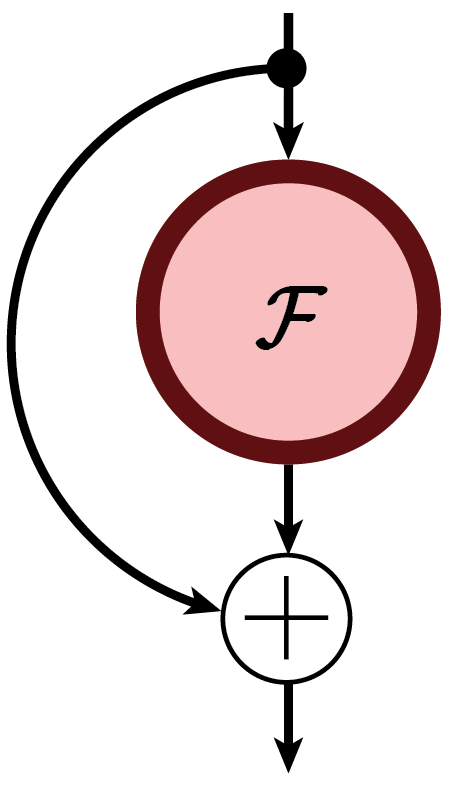
\includegraphics[width=0.13\textwidth]{\imgpath/resnet.png}
  }\qquad
  \subfloat[Lifting]{
  \centering
  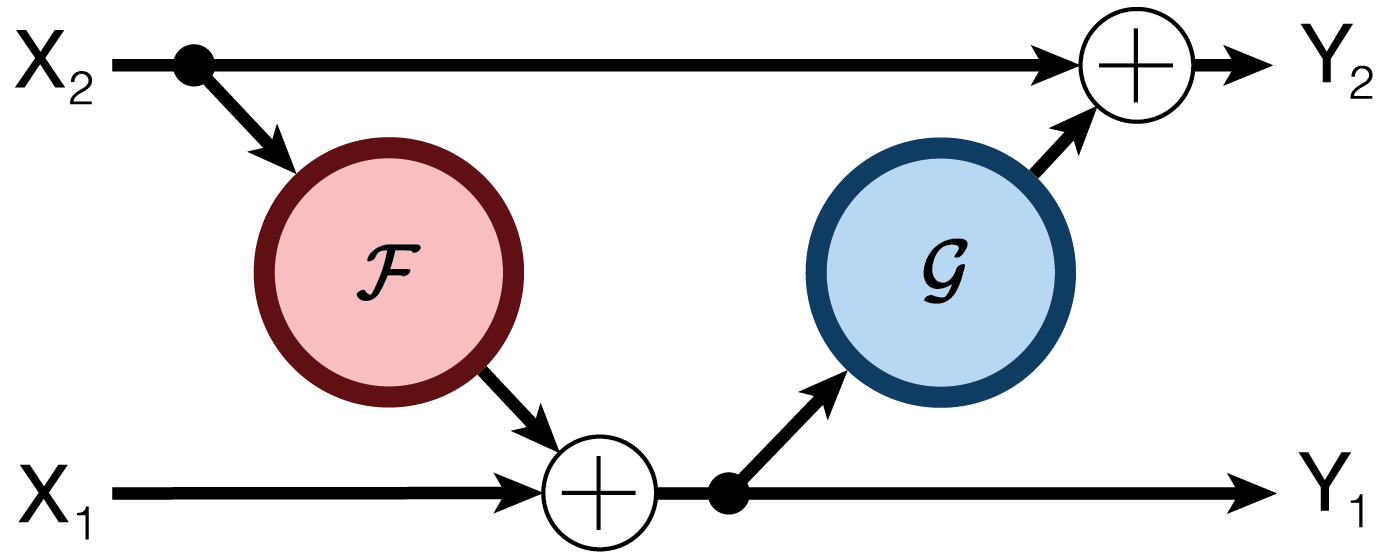
\includegraphics[width=0.48\textwidth]{\imgpath/lifting.png}
  }
  \mycaption{Residual vs Lifting Layers}{In a residual layer, an input is
  transformed by a learned function $\mathcal{F}$ and added to itself. Typically
  $\norm{\mathcal{F}x} \ll \norm{x}$ meaning the vector $y$ is a small
  perturbation of the vector $x$. In a lifting layer, each path is a learned
  function of the other added to itself. In the original second generation
  wavelets, $\mathcal{F}$ and $\mathcal{G}$ are FIR filters, but there is no
  requirement on them to be.}
  \label{fig:ch7:lifting_resnet}
\end{figure}
We briefly mentioned ResNets in \autoref{sec:ch2:resnets} but did not study them
in depth in this thesis. Interestingly, there are many similarities between
ResNets and second generation wavelets, or the \emph{lifting} framework
\cite{sweldens_lifting_1998,daubechies_factoring_1998}.
In a residual layer, the output is $y = \mathcal{F}(x) + x$, for a lifting
system, the layer is a two port network:
\begin{align}
  y_1 &= \mathcal{F}(x_1) + x_2 \\
  y_2 &= \mathcal{G}(y_1) + x_1 
\end{align}
\autoref{fig:ch7:lifting_resnet} shows the similarities between the two designs. 
\cite{gomez_reversible_2017, jacobsen_i-revnet:_2018} both make the small modifications
to the ResNet design to make a lifting style architecture.
\cite{gomez_reversible_2017} do this to save memory on the activations for
backpropagation whereas \cite{jacobsen_i-revnet:_2018} use it for its perfect
reconstruction properties. We believe that there are potentially many more
benefits to using the lifting design as an extension of our work into learning
from basis functions.

In addition to the interesting parallel between ResNets and Lifting,
\citeauthor{bartlett_gradient_2018} have found that having near identity transforms
for each stage of a deep learning system is \cite{bartlett_gradient_2018, bartlett_representing_2018}
Aside from the interesting parallel between ResNets and Lifting, ResNets have
become 
\subsection{Protecting against Attacks}
\cite{cisse_parseval_2017}

\subsection{Convolutional Sparse Coding}

\cite{liu_online_2017, liu_first_2017, papyan_convolutional_2017}

\subsection{Energy Propagation and Weight Properties}
studying the energy propagation properties and singular values of layers

Miki Elad's work on CSC.

ResNets are really good. What was the paper on that?
(Bartlett


